\documentclass{llncs}
\pagestyle{plain}
\usepackage[show]{ed}
\usepackage[utf8]{inputenc}
\usepackage{xspace}
\usepackage{amssymb}
\usepackage{wrapfig}
\usepackage[style=alphabetic,backend=bibtex,isbn=false]{biblatex}
\addbibresource{../../lib/kbibs/kwarcpubs.bib}
\addbibresource{../../lib/kbibs/extpubs.bib}
\addbibresource{../../lib/kbibs/kwarccrossrefs.bib}
\addbibresource{../../lib/kbibs/extcrossrefs.bib}
\addbibresource{rest.bib}% add bibs here!
\renewbibmacro*{event+venue+date}{}
\renewbibmacro*{doi+eprint+url}{%
  \iftoggle{bbx:doi}
    {\printfield{doi}\iffieldundef{doi}{}{\clearfield{url}}}
    {}%
  \newunit\newblock
  \iftoggle{bbx:eprint}
    {\usebibmacro{eprint}}
    {}%
  \newunit\newblock
  \iftoggle{bbx:url}
    {\usebibmacro{url+urldate}}
    {}}

% identifiers and URIs
\providecommand{\identifier}[1]{%
  \StrSubstitute{#1}{\_}{_}[\identifiertmp]
  \expandafter\path\expandafter{\identifiertmp}%
}
\let\uri\identifier

% Jay, tables
\usepackage{tabularx}
\usepackage{multirow}

% TIKZ
\usepackage{tikz}
\def\thmo#1#2{\mathsf{#1}\colon\kern-.15em{#2}}% for theories
\usetikzlibrary{shapes,arrows,mmt,fit,shadows}

% Abbreviations
\providecommand{\mmt}{MMT}
\providecommand{\omdocmmt}{OMDoc/MMT}
\providecommand{\lmfdb}{LMFDB}

% colors for syntax highlighting
\usepackage{xcolor}
\colorlet{punct}{red!60!black}
\definecolor{background}{HTML}{EEEEEE}
\definecolor{delim}{RGB}{20,105,176}
\colorlet{numb}{magenta!60!black}

% code snippets
\usepackage{listings}
% QMT
\lstdefinelanguage{qmt}{
    basicstyle=\footnotesize\ttfamily,
    showstringspaces=false,
    frame=single, 
    mathescape, 
    columns=fullflexible,
    breaklines=true
}
% JSON syntax
\lstdefinelanguage{json}{
    basicstyle=\footnotesize\sffamily,
    numberstyle=\scriptsize,
    showstringspaces=false,
    breaklines=true,
    frame=single, 
    literate=
     *{0}{{{\color{numb}0}}}{1}
      {1}{{{\color{numb}1}}}{1}
      {2}{{{\color{numb}2}}}{1}
      {3}{{{\color{numb}3}}}{1}
      {4}{{{\color{numb}4}}}{1}
      {5}{{{\color{numb}5}}}{1}
      {6}{{{\color{numb}6}}}{1}
      {7}{{{\color{numb}7}}}{1}
      {8}{{{\color{numb}8}}}{1}
      {9}{{{\color{numb}9}}}{1}
      {:}{{{\color{punct}{:}}}}{1}
      {,}{{{\color{punct}{,}}}}{1}
      {\{}{{{\color{delim}{\{}}}}{1}
      {\}}{{{\color{delim}{\}}}}}{1}
      {[}{{{\color{delim}{[}}}}{1}
      {]}{{{\color{delim}{]}}}}{1},
}

\providecommand{\inlinecode}[1]{{\lstinline[language=qmt]|#1|}}

\def\meta#1{\ensuremath{\langle\kern-.25em\langle}#1\ensuremath{\rangle\kern-.2em\rangle}}

% More abbreviatons for diagrams and things
\def\plaintt#1{\ifmmode\mathrm{\texttt{#1}}\else\texttt{#1}\fi}
\def\typett{\plaintt{type}}
\def\codectt{\plaintt{codec}}


\usepackage{hyperref}
\title{REGULAR-T1: Virtual Theories -- A Uniform Interface to Mathematical Knowledge Bases}
\author{
Tom Wiesing\inst{1}
Michael Kohlhase\inst{1} 
Florian Rabe\inst{2} 
}

\institute{
   FAU Erlangen-N\"urnberg
   \and Jacobs University Bremen
%   \and Universit\'e Paris-Sud
}
\begin{document}
\maketitle
\begin{abstract}
  There are various mathematical knowledge collections and information systems available. 
  They range from completely informal ones like Wikipedia or the Cornell arXiv, zbMath, and MathSciNet via mathematical object databases like the GAP group libraries, the Online Encyclopedia of Integer sequences (OEIS), and the L-functions and Modular Forms Database (LMFDB) to theorem prover libraires like those of Mizar, Coq, PVS, and the HOL systems. 

  Unfortunately, these systems are often only accessible via a dedicated web information system or a low-level API at the level of the raw database content. 
  What we would want is a ``programmatic, mathematical API'' which would give access to the knowledge-bases programmatically via their mathematical constructions and properties. 

  This paper takes a step into this direction by interpreting knowledge bases as \omdocmmt\ theory graphs -- modular, flexiformal representations of mathematical objects, their properties, and relations. 
  We update \omdocmmt\ theories to ``virtual theories'' and update knowledge management algorithms so that they can cope with theories that do not fit into main memory but directly deal with the underlying databases as backends employing a modular system of codecs to bridge the gap between the database schema and the mathematical construction of objects.
\end{abstract}

%\ednote{Target Size: 15 pages}

\section{Introduction}\label{sec:intro}

\begin{newpart}{MK: adapted from Tom's Thesis}
There is a large and vibrant ecosystem of open-source mathematical software systems.
These systems can range from calculators, which are only capable of performing simple
computations, via mathematical databases (curating collections of a mathematical objects)
to powerful modeling tools and computer algebra systems (CAS). 

Most of these systems are very specific -- they focus on one or very few aspects of
mathematics.  For example, the ``Online Encyclopedia of Integer Sequences''
(OEIS~\cite{Sloane:oeis12,oeis}) focuses on sequences over $\mathbb{Z}$ an their
properties and the ``L-Functions and Modular Forms Database''
(LMFDB)~\cite{Cremona:LMFDB16,lmfdb:on} objects in number theory pertaining to Langland's
program.  GAP~\cite{GAP:on} excels at discrete algebra, whereas
SageMath~\cite{SageMath:on} focuses on Algebra and Geometry in general, and
Singular~\cite{singular:on} on polynomial computations, with special emphasis on
commutative and non-commutative algebra, algebraic geometry, and singularity theory.

For a mathematician however (a user; let us call her Jane) the systems themselves are not relevant, instead she only cares about being able to solve problems. 
Typically, it is not possible to solve a mathematical problem using only a single program. 
Thus Jane needs to work with multiple systems and combine the results to reach a solution. 
Currently there is very little help with this practice, so Jane has to isolate sub-problems the respective systems are amenable to, formulate them into the respective input language, collect results, and reformulate them for the next system a tedious and error-prone process at best, a significant impediment to scientific progress in its overall effect. 
Solutions for some situations certainly exist, which can help get Jane unstuck, but these are ad-hoc and for specific, often-used system combinations only. 
Each of these requires a lot of maintenance and does not scale to a larger set of specialist systems. 

The OpenDreamKit project, which aims at a mathematical VRE toolkit, proposes the Math-in-the-Middle (MitM~\cite{DehKohKon:iop16}) Paradigm, an interoperability framework based on a flexiformal
representation of mathematical knowledge and aligns this with system-generated interface
theories. 

In this paper we instantiate the MitM paradigm with a concrete domain development and
evaluate it on a distributed computing GAP, SageMath and Singular.\ednote{ we generally we
  want to show that the promises in the CICM paper become reality.}

We will use the following example as a running example: Jane wants to act on singular
polynomials with GAP permutation groups\ednote{MK@(MP|VA): }

 \ednote{MK: continue with the structure} 
\end{newpart}

%%% Local Variables:
%%% mode: latex
%%% TeX-master: "paper"
%%% End:

\section{Virtual Research Environments for Mathematics: the Math-in-the-Middle
  Approach}\label{sec:mmtmitm}

The work reported in this paper originates from in the EU-funded OpenDreamKit
\cite{OpenDreamKit:on} project that aims to create Virtual Research Environments (VRE)
enabling mathematicians to make efficient use of existing Open-Source mathematical
knowledge systems.  These systems include computer algebra systems like SageMath and GAP
as well as mathematical data bases such as the \lmfdb, which must be made interoperable
for integration into a VRE. In the OpenDreamKit project we have developed the
Math-in-the-Middle (MitM) approach, which posits a central ontology of mathematical
knowledge, which acts as a pivot point for interoperability; see~\cite{DehKohKon:iop16}
for a description of the approach and \cite{KohMuePfe:kbimss17} for a technical refinement
and large-scale interoperability case study. 

\begin{wrapfigure}l{0.3\textwidth}%\vspace*{-2em}
    \begin{tikzpicture}[xscale=1.3,yscale=1.3]\normalsize
      \tikzstyle{withshadow}=[draw,drop shadow={opacity=.5},fill=white]
      \tikzstyle{system}=[draw]
      \tikzstyle{standard}=[circle,fill=blue!30]
      \tikzstyle{interface}=[circle,fill=purple!30,inner sep = 1pt,]
      \node[system] (a) at (0,.3) {A};
      \node[system] (b) at (1,.3) {B};
      \node[system] (c) at (1.7,1) {C};
      \node[system] (d) at (1.7,2) {D};
      \node[system] (e) at (1,2.7) {E};
      \node[system] (f) at (0,2.7) {F};
      \node[system] (g) at (-.7,2) {G};
      \node[system] (h) at (-.7,1) {H};
      \node[standard] (m) at (.5,1.5) {S};
      \node[interface] (ia) at (0.2,.9) {a};
      \node[interface] (ib) at (.8,.9) {b};
      \node[interface] (ic) at (1.1,1.2) {c};
      \node[interface] (id) at (1.1,1.75) {d};
      \node[interface] (ie) at (.8,2.1) {e};
      \node[interface] (if) at (0.2,2.1) {f};
      \node[interface] (ig) at (-.1,1.75) {g};
      \node[interface] (ih) at (-.1,1.2) {h};
      \draw (m) -- (ia) -- (a);
      \draw (m) -- (ib) -- (b);
      \draw (m) -- (ic) -- (c);
      \draw (m) -- (id) -- (d);
      \draw (m) -- (ie) -- (e);
      \draw (m) -- (if) -- (f);
      \draw (m) -- (ig) -- (g);
      \draw (m) -- (ih) -- (h);
      \end{tikzpicture}
  \caption{The MiTM Approach to Connecting Systems.}\label{fig:mitmconnect}\vspace*{-1em}
\end{wrapfigure}
The MitM ontology in the center of Figure~\ref{fig:mitmconnect} models the true,
underlying mathematical semantics in \ommt and allows translation between this centrally
formalized knowledge and the systems on the boundary via views and alignments.
This mathematical knowledge is modeled using the well-established theory graph paradigm
and is stored inside our \ommt-based MathHub system~\cite{MathHub:on}. 

The knowledge in the mathematical software systems -- denoted by square boxes in
Figure~\ref{fig:mitmconnect} -- also modeled via \ommt theory graphs the \textbf{API
  Content Dictionaries} -- the corresponding red circles; these are generated from the
knowledge bases in the systems by a custom process. The API CDs allow us to implement
translation with the help of \ommt views and alignments between the ontology -- the
Math-In-The-Middle -- and each of the systems and use these translations for transporting
computational tasks between the systems. 

The realization of the MitM approach crucially depends on the information architecture of
the \ommt language~\cite{Kohlhase:OMDoc1.2,RabKoh:WSMSML13} and its implementation in the
\mmt system~\cite{Rabe:MAGMS13,uniformal:on}.

In \ommt knowledge is organized in \textbf{theories}, which contain information about
mathematical concepts and objects in the form of \textbf{declarations}. Theories are
organized into an ``object-oriented'' inheritance structure via \textbf{inclusions} and
\textbf{structures} (for controlled multiple inheritance), which is augmented via
truth-preserving mappings between theories called \textbf{views}, which allow to relate
concepts of pre-existing theories and transport theorems between these. Inclusions,
structures, and views impose a graph structure on the represented mathematical knowledge,
called a \textbf{theory graph}. 

We observe that even very large mathematical knowledge spaces about abstract mathematical
domains can be represented by small, but densely connected, theory graphs, if we make all
inherited material explicit in a process called \textbf{flattening}. The \ommt language
provides systematic names (\mmt URIs) for all objects, properties, and relations in the
induced knowledge space, and given the represented theory graph, the \mmt system can
compute them by need. 

Generally, knowledge in a knowledge space given by a theory graph loaded by the \mmt
system can be accessed by either giving it's \mmt URI, or by giving a set of conditions
that has to fulfilled by the knowledge in question. The achieve the latter, \mmt has a
Query Language called QMT~\cite{Rabe:qlfml12}, which allows even complex conditions to be
specified. Concretely, the \mmt system loads the theory graph into main memory at startup
and interleaves incremental flattening and query evaluation operations on the \mmt data
structures until the result has been produced. 

In \cite{KohMuePfe:kbimss17} we show that the MitM approach, its \ommt-based realization,
and distribution via the SCSCP protocol are sufficient distributed, federated computation
between multiple computer algebra systems (Sage, GAP, and Singular), and that the MitM
ontology of abstract group theory can be represented in \ommt efficiently. This setup is
effective because
\begin{compactenum}[\bf C1]
\item the knowledge spaces behind abstract and computational mathematics can be
  represented in theory graphs very space-efficiently: The compression factors between a
  knowledge space and its theory graph -- we call it the \textbf{TG factor}\ednote{MK@FR:
    we should have a name for that factor; something like the ``deBruijn factor''; only
    that we want it to be large! I think we should talk about this on the tetrapod meeting
    and jointly decide on one and argue with that; I will use TG factor for now.} --
  exceed two orders of magnitude even for small domains.
\item only small parts of the knowledge space are traversed for a given computation. 
\end{compactenum}

But the OpenDreamKit VRE must also include mathematical data sources like the \lmfdb or
the OEIS, which contain millions of mathematical objects. For such knowledge sources, the
classical \mmt system is not yet suitable: 
\begin{compactenum}[\bf V1]
\item the knowledge space corresponding to the data base content cannot be compressed by
  ``general mathematical principles'' like inheritance. Indeed, redundant information is
  already largely eliminated by the data base schema and the ``business logic'' of the
  information system.
\item typically large parts of the knowledge space need to be traversed to obtain the
  intended results to queries.
\end{compactenum}
As a consequence, we extend the concept of \ommt theories -- which carry the implicit
assumption of containing only a small number of declarations (see~\cite{FaGu:lt92} for a
discussion) -- to \textbf{virtual theories}, which can have an unlimited number of
declarations or -- while we are at it -- even infinitely many. To contrast the intended
uses we will call the classical \ommt theories \textbf{concrete theories}. 

From a system perspective, virtual theories behave just like concrete theories, but
without the assumption of loading all declarations from a file on disk at system startup.
Instead of loading all knowledge from an XML file, virtual theories load declarations in a
lazy fashion when they are required.  Here we do not even restrict ourselves to lazily
reading an XML file, on the contrary, in most use cases we actually create the \ommt
representation on demand.

%%% Local Variables:
%%% mode: latex
%%% TeX-master: "paper"
%%% End:

%  LocalWords:  omdocmmt fig:classicalconnect fig:mitmconnect OpenDreamKit:on lmfdb lmfdb
%  LocalWords:  ODKproposal:on DehKohKon:iop16 sagemath oeis fig:mitmontology colored ig
%  LocalWords:  mathrm mathrm sec:mmtmitm ommt mechanized uniformal:on organized textit
%  LocalWords:  BusCapCar:oms04 MathHub:on Iancu:phd SMGloM:on formalizations wrapfigure
%  LocalWords:  PVSlibraries:on mizar:online textwidth tikzpicture xscale 1.3,yscale
%  LocalWords:  tikzstyle withshadow draw,drop circle,fill 30,inner formalized vspace
%  LocalWords:  MACIS17-interop KohMuePfe:kbimss17 1.3,yscale 30,inner fit:mitmconnect
%  LocalWords:  textbf realization RabKoh:WSMSML13 Rabe:MAGMS13,uniformal:on Rabe:qlfml12
%  LocalWords:  FaGu:lt92

\section{Example: The API and Structure of LMFDB}\label{sec:sota}

The ``L-Functions and Modular Forms Database'' (\lmfdb~\cite{lmfdb}) is a large database, storing among other mathematical objects several thousand L-Functions and curves along with their properties. 
Technically, it uses a MongoDB database with a Python web frontend. 
We use this as an example of a virtual theory. 
Before we go into this in more detail, we have a closer look at the structure and existing APIs to of \lmfdb.

\subsection{The Structure of LMFDB}\label{sec:sota:struct}

\lmfdb has several sub-databases, e.g., for elliptic curves or transitive groups. 
Within each of these, every object is stored as a single JSON record.
Figure~\ref{fig:lmfdbexample} shows an example: each property of this JSON object corresponds to a property of the underlying mathematical object. 
For example, the \identifier{degree} property -- here $1$ -- of the JSON objects corresponds to the degree of the underlying elliptic curve. 

\begin{figure}[ht]\centering
\begin{lstlisting}[language=json]
{
    "degree": 1,
    "x-coordinates_of_integral_points": "[5,16]",
    "isogeny_matrix": [[1,5,25],[5,1,5],[25,5,1]],
    "label": "11a1",
    "_id": "ObjectId('4f71d4304d47869291435e6e')",
    ...
}
\end{lstlisting}\vspace*{-1.5em}
  \caption[An elliptic curve from \lmfdb]{
    Part of an elliptic curve in \lmfdb (some fields omitted for brevity)
  }
  \label{fig:lmfdbexample}
\end{figure}

Other properties are more complex: the value of the \identifier{isogeny\_matrix} property is a list of lists representing a matrix. 
This disconnect between JSON encoding and mathematical meaning can become much more severe, e.g., the \identifier{x-coordinates\_of\_integral\_points} field is semantically a list of integers but (due to the sizes limits on integers) is encoded as a string.

\subsection{An API for \lmfdb Objects}\label{sec:sota:api}

\begin{wrapfigure}r{0.7\textwidth}\centering\vspace*{-2.5em}
  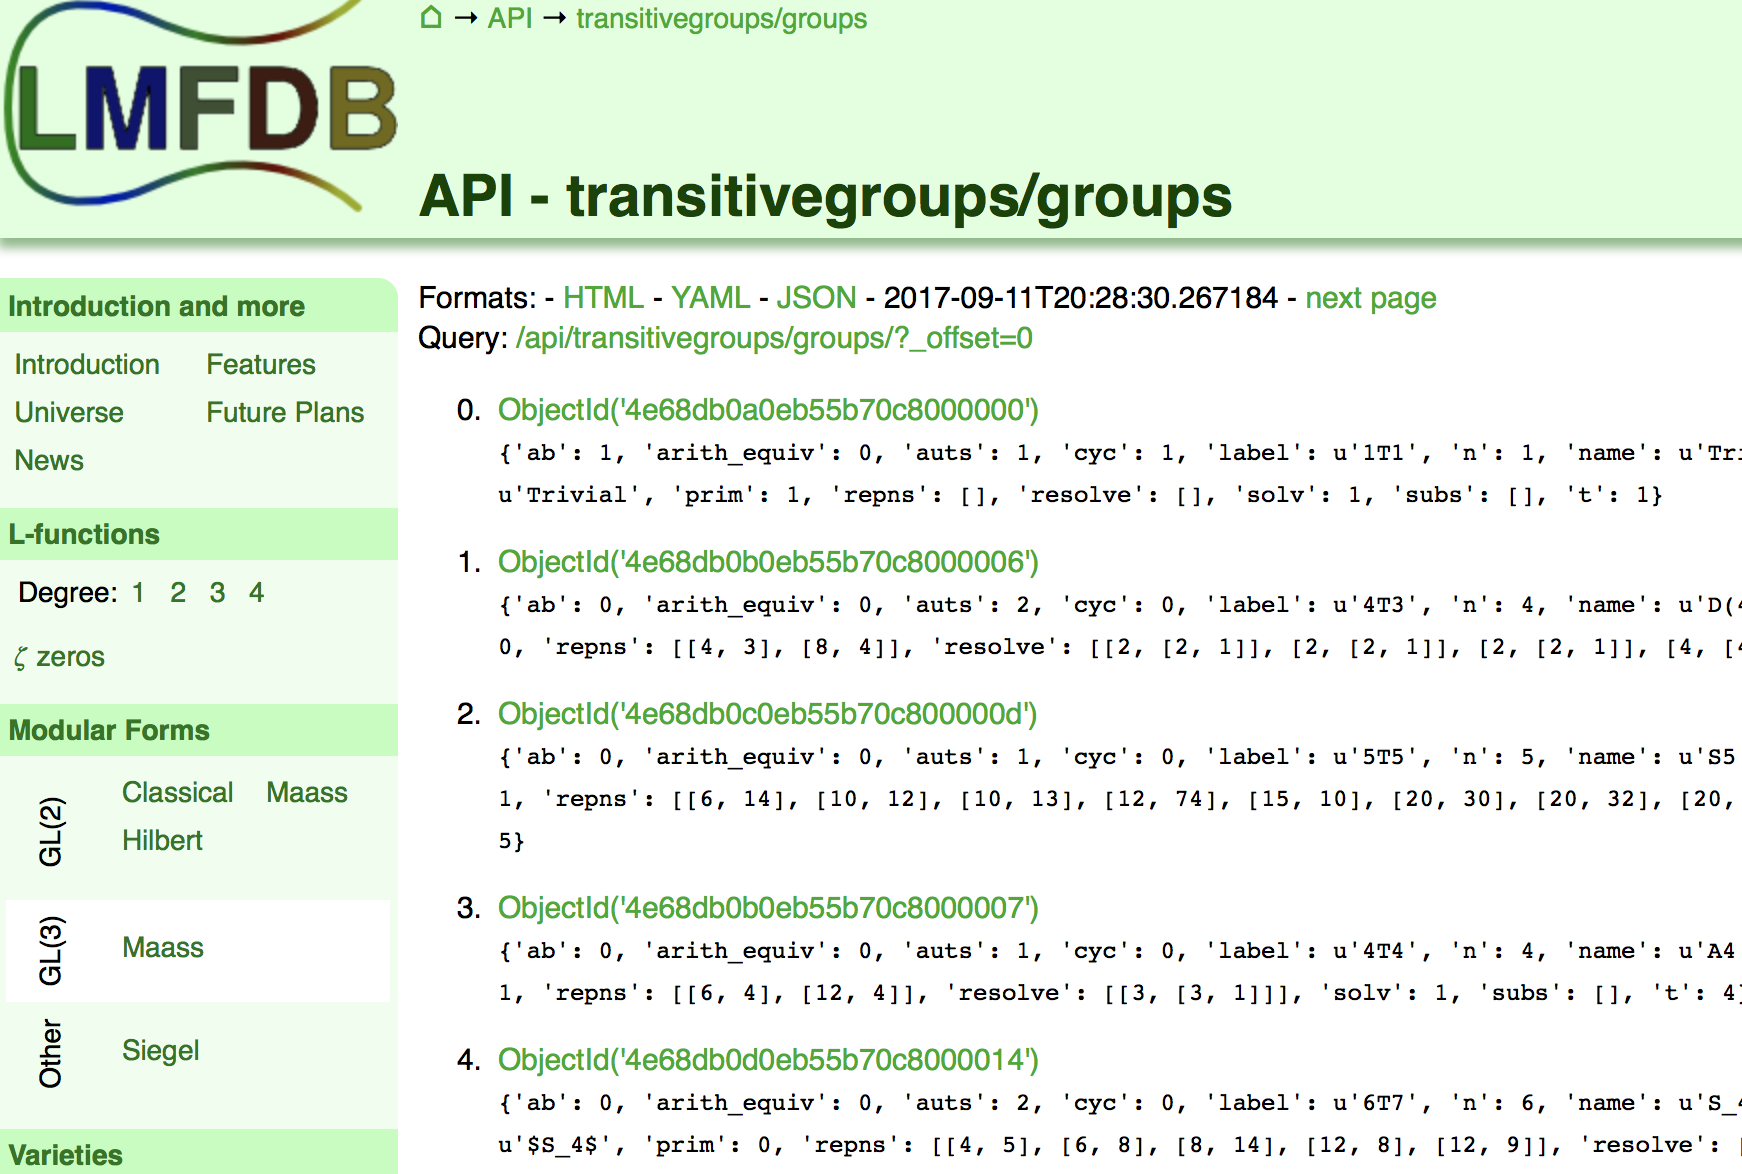
\includegraphics[width=0.7\textwidth]{APIScreenshot}
  \caption[The Web-Interface for the \lmfdb API. ]{
    The Web-Interface for the \lmfdb API. 
  }\vspace*{-1.5em}
  \label{fig:apiscreenshot}
\end{wrapfigure}
Querying is an important application for mathematical knowledge bases.
The \lmfdb API \cite{lmfdbapi} exposes a querying interface that can be used either by humans via the web or programmatically via JSON-based GET requests.
A screenshot of the former interface can be seen in Figure~\ref{fig:apiscreenshot}. 

Queries must name the sub-database to be queried and consist of a set of key-value pairs that correspond to an SQL \texttt{where} clause.
However, while \lmfdb offers a programmable API for accessing its contents, this API sits at the level of the underlying MongoDB, and not the level of mathematical objects. 
For example, to retrieve all Abelian objects in the subdatabase of transitive groups, we expect to use the key-value pair \identifier{commutative}$ = $ \identifier{true}. 
However, these values need to be encoded to be understood by MongoDB.
We need to realize that the database schema actually uses the key \identifier{ab} for commutativity, that it has boolean values, and that the schema encodes \inlinecode{true} as \inlinecode{1}. 
Thus, the actual query to send is \url{http://www.lmfdb.org/api/transitivegroups/groups/?ab=1}. 

In this example, all steps are relatively straightforward. 
But in general, e.g. when searching for all elliptic curves with a specific isogeny matrix, this not only requires good familiarity with the mathematical background but also with the system internals of the particular \lmfdb sub-database; a skill set commonly found in neither research programmers nor average mathematicians.   

Our diagnosis is that {\lmfdb} -- and most other mathematical knowledge databases -- suffer from two problems:
\begin{compactitem}
\item \emph{human/computer mismatch}: humans have problems interacting with \lmfdb because they must speak the system language instead of mathematical language
\item \emph{computer/computer mismatch}: mathematical computer systems cannot interoperate with \lmfdb because their system languages differ.
\end{compactitem}
Using the MitM approach we have presented in Section~\ref{sec:mmtmitm}, we can solve both problems at the same time by lifting the communication to the level of \ommt-encoded MitM objects, which both MitM-compatible software systems and humans can understand.
%%% Local Variables:
%%% mode: latex
%%% TeX-master: "paper"
%%% End:

%  LocalWords:  sec:sota lmfdb lmfdb lstlisting json ainvs iwp0 2adic_gens isogeny_matrix
%  LocalWords:  tamagawa_product 2adic_index anlist 4f71d4304d47869291435e6e vspace emph
%  LocalWords:  fig:lmfdbexample isogeny includegraphics textwidth fig:apiscreenshot
%  LocalWords:  centering summarize sec:mmtmitm ommt-encoded 4f71d4304d47869291435e6e
%  LocalWords:  serialization wrapfigure

% !TEX root = ../thesis.tex
\section{Using Codecs To Implement \lmfdb Virtual Theories}\label{sec:vt}

From a system perspective, virtual theories behave just like concrete theories, but
without the assumption of loading all declarations from a file on disk at system startup.
Instead, virtual theories load declarations in a lazy fashion when they are
needed. Concrete theories are stored as XML files; i.e. we use the file system as a
backend for the \mmt system. As most of the knowledge sources we want to embed into \ommt
as virtual theories use data-bases as back-ends and provide low-level database APIs we
have extended the \mmt backends for this as well. Apart from standard software engineering
tasks, there were three conceptual problems to be solved in this extension/implementation:
\begin{compactenum}[\bf P1]
\item How to match the database tables into \ommt theories and declarations. 
\item How to lift data in \textbf{physical representation} -- i.e. as records of the
  underlying database to \ommt terms -- i.e. data in \textbf{semantic representation}.
\item And how to translate QML queries from semantic to physical representation -- i.e. so
  that they can be executed directly on the data base without loading bulk data into the
  \mmt process.
\end{compactenum}
We will discuss all three using the \lmfdb case discussed above as a running
example. \textbf{P1} can only be solved for each concrete application: Generally, we need
to represent \lmfdb as a set of \ommt theories.  As each sub-database in \lmfdb contains
records of similar structure, it makes sense to create a single virtual theory for each of
these sub-databases and use \ommt declarations for each of the objects. We address
\textbf{P2} next.

\subsection{Translating between Physical and Semantic Representations}\label{sec:vt:translation}

Consider, for example the \identifier{degree} field from the example above.  We have
already seen that this represents the degree of a curve and is an integer value, in this
case the integer $1$.  As \lmfdb uses MongoDB, which is based on JSON, integer values will
usually be represented as a JSON numbers, i.e. an \identifier{IEEE 754} $64$ bit floating
point number.  Here this is the floating point value $1.0$. But when the semantic
representations can exceed the have a maximum possible value $2^{53}-1$ of IEEE floats,
\lmfdb uses a different encoding, e.g. JSON strings that have no hard upper limit.

Let us call the set of objects in semantic representation the \textbf{semantic type}, and
the set of objects in the physical representation the \textbf{realized type}.  Semantic
types reside in the MiTM ontology, whereas realized types resides in the systems
themselves. Corresponding with intuition, the process of converting between the two
representations is called \textbf{coding}, specifically coding into a semantic
representation is called \textbf{encoding}, the reverse is called \textbf{decoding}. We
will call system components that do the necessary translation -- \underline{co}ding and
\underline{dec}oding -- \textbf{CoDec}s. 

As \ommt is a typed framework, we can directly use \ommt types from the MitM ontology for
the semantic types. Simple realized types are usually atomic database types whereas
complex realized types correspond to database tables or views; the details of this setup
are determined by the database schema. To arrive at a tight integration with the \ommt
functionality we will represent as much of this information in \ommt as possible.

Therefore we introduce a new \ommt theory \texttt{Codecs} in the foundational part of the
MitM ontology. See Figure~\ref{fig:vtarch} for details how this plays in the overall
information architecture and Figure~\ref{fig:codecs} for elementary content. This theory
introduces a type constructor \codectt, which given a semantic type constructs the type of
codecs for this type. For instance, the object \identifier{StandardPos} is (a CoDec) of
type $\codectt\;\mathbb{Z}^+$, i.e. a CoDec that parses database objects (for \lmfdb a
IEEE floats) into \ommt terms that can be typed as MitM positive integers and serializes
them back.

\begin{figure}[ht]\centering
  \begin{tikzpicture}\footnotesize
    \node[thy] (codecs) at (0,0) {
      \begin{tabularx}{.84\textwidth}{lll|X}
        \multicolumn{4}{l}{\textsf{Codecs}} \\\hline\hline   
        \identifier{codec}    & : & \multicolumn{1}{l}{$\typett\rightarrow\typett$} & \\\hline
        \identifier{StandardPos}    & : & $\codectt\; \mathbb{Z}^{+}$   & \multirow{3}{*}{\begin{minipage}{3.8in}
                                                                                      JSON number if small enough, \\
                                                                                      else JSON string of decimal expansion
                                                                                      \end{minipage}}\\
        \identifier{StandardNat}    & : & $\codectt\; \mathbb{N}$       & \\
        \identifier{StandardInt}    & : & $\codectt\; \mathbb{Z}$       & \\\hline
        \identifier{IntAsArray}     & : & $\codectt\; \mathbb{Z}$       & JSON List of Numbers\\
        \identifier{IntAsString}    & : & $\codectt\; \mathbb{Z}$       & JSON String of decimal expansion\\\hline
        \identifier{StandardBool}   & : & $\codectt\; \mathbb{B}$       & JSON Booleans \\
        \identifier{BoolAsInt}      & : & $\codectt\; \mathbb{B}$       & JSON Numbers $0$ or $1$ \\\hline
        \identifier{StandardString} & : & $\codectt\; \mathbb{S}$       & JSON Strings \\
      \end{tabularx}
    };
  \end{tikzpicture}
  \caption[List of Codecs]{
    An annotated subset of the Codecs theory containing a selection of codecs found in \mmt. 
    Here $\mathbb{N}$ represents natural numbers (including $0$), 
    $\mathbb{Z}$ integers, 
    $\mathbb{Z}^{+}$ positive integers, 
    $\mathbb{B}$ booleans and
    $\mathbb{S}$ (unicode character) strings. 
  }
  \label{fig:codecs}
\end{figure}
The \identifier{degree} we used as an example above would use the \identifier{StandardInt}
codec. Additionally the \textsf{CoDecs} theory associates with each codec a Scala class
that implements the translation between semantic and realized type.

But codecs for basic types (semantic and realized) is not sufficient for our application.
Consider for example the \identifier{isogeny\_matrix} field of an elliptic curve
representation.  The semantic representation of the value of this field is the matrix
\[M = \left(
    \begin{array}{ccc}
      1 & 5 & 25 \\
      5 & 1 & 5 \\
      25 & 5 & 1 \end{array} 
  \right)
\]
Matrices are characterized with three parameters, the type of object they contain
(integers in this case) along their row and column count ($3 \times 3$ in this case).  In
principle, one could construct a codec for each type of matrices by hand.  This would mean
generating one codec for $1 \times 1$ integer matrices, $1 \times 1$ real matrices,
$1 \times 2$ integer matrices, $1 \times 2$ real matrices, and so on.  For the
representation of codecs in \mmt, this would require generating one symbol and one Scala
function for each different kind of matrix.  This quickly becomes a mess.

Instead we use the fact that both Scala and \ommt allow higher-order functions: We can
define a \textbf{codec operator} that given a codec the parameter type $\tau$ and values
for the number $n$ of rows and $m$ of columns, generate a codec of $n\times m$ matrices of
$\tau$ objects. In the example above and the matrix $M$ is encoded as a list of $n$ lists
of $m$ integers ($\tau$):
% HACK HACK HACK overfull box\\\noindent
\inlinecode{[[1.0,5.0,25.0],[5.0,1.0,5.0],[25.0,5.0,1.0]]}

\begin{figure}[ht]\centering
  \begin{tikzpicture}\footnotesize
    \node[thy] (codecs) at (0,0) {
      \begin{tabularx}{\textwidth}{lll|X}
        \multicolumn{4}{l}{\textsf{Codecs (continued)}} \\\hline\hline   
        \identifier{StandardList}    & : & 
                 $\left\{T\right\} \codectt\; T \rightarrow \codectt\; \mathrm{List}(T)$ & 
                  JSON list, recursively coding each element of the list\\\hline
        \identifier{StandardVector}    & : & 
                  $\left\{T, n\right\} \codectt\; T \rightarrow \codectt\; \mathrm{Vector}(n, T)$ & 
                   JSON list of fixed length $n$\\\hline
        \identifier{StandardMatrix}    & : & 
                   $\left\{T, n, m\right\} \codectt\; T \rightarrow \codectt\; \mathrm{Matrix}(n, m, T)$ & 
                   JSON list of $n$ lists of length $m$\\
      \end{tabularx}
    };
  \end{tikzpicture}
  \caption[List of Codec Operators]{
    Second annotated subset of the codecs theory containing a selection of codec operators found in \mmt. 
    Compare with Figure~\ref{fig:codecs}. 
  }
  \label{fig:codecops}
\end{figure}
Like first-order codecs, codec operators in \mmt are again represented in two ways, as
declarations inside the \identifier{CoDecs} theory (see Figure~\ref{fig:codecops} for a
list) and as a corresponding Scala implementation -- a higher-order function from CoDecs
to CoDecs. This is mirrored in the types of operators in Figure~\ref{fig:codecs}: the
\textsf{StandardMatrix} operator is a function that takes four arguments: a type $T$, two
numbers $n$ and $m$, and a $\tau$-codec and yields a $\mathrm{Matrix}(n, m,
T)$-codec. Here we make use of the dependent function types of the MitM foundation:
arguments in curly brackets can be used in the result type; see~\cite{RabKoh:WSMSML13} for
details.

With these declarations in the \textsf{CoDecs} theory, we can represent a codec for
$3 \times 3$ integer matrices e.g. for the the isogeny matrix $M$ above by the \ommt term
$\plaintt{StandardMatrix}(3, 3, \plaintt{StandardInt})$\footnote{The observant reader will
  have noticed that the way codec operators have been declared, the codec in question
  actually corresponds to the term
  $\plaintt{StandardMatrix}(\mathbb{Z}, 3, 3, \plaintt{StandardInt})$.  This has an
  additional $\mathbb{Z}$ as the first argument.  However, the last argument is a codec
  for a specific semantic type and thus fully determines the first argument.  \mmt is
  capable of transparently inferring the first argument, thus it can be omitted for
  readability without needing any kind of special treatment implementation wise.  }.
Similarly the same codec operator can be used to for example generate a codec for
$2 \times 2$ boolean matrices, which corresponds to
$\plaintt{StandardMatrix}(2, 2, \plaintt{StandardBool})$.

\subsection{Schema Information in Virtual Theories}\label{sec:vt:schemas}

\begin{figure}[ht]\centering
    \begingroup
    \pgfdeclarelayer{background}
    \pgfdeclarelayer{foreground}
    \pgfsetlayers{background,foreground}
    
    \resizebox{\textwidth}{0.75\textwidth}{
      \begin{tikzpicture}[xscale=4,yscale=3]\footnotesize
        \begin{pgfonlayer}{foreground}
          \tikzstyle{human}    = [red,dashed,thick]
          \tikzstyle{withshadow}  = [draw,drop shadow={opacity=.5},fill=white]
          \tikzstyle{interface}   = [fill=blue!30]
          \tikzstyle{database}    = [cylinder,cylinder uses custom fill,
            cylinder body fill=yellow!50,cylinder end fill=yellow!50,
            shape border rotate=90,
            aspect=0.25,draw]
          
          % Ontology layer
          \node[thy] (numbers) at (0,1) {
            \begin{tabular}{lll}
              \multicolumn{3}{l}{\textsf{Numbers}}\\\hline\hline
              $\mathbb{Z}^{+}$        & : & \typett\\
              $\mathbb{Z}$            & : & \typett\\\hline
              \multicolumn{3}{l}{$\mathbb{Z}^{+} \subset \mathbb{Z}$}
            \end{tabular}
          };

          \node[thy] (matrices) at (1.5,1) {
            \begin{tabular}{lll}
              \multicolumn{3}{l}{\textsf{Matrices}}\\\hline\hline
              \plaintt{matrix} & : & $\typett \rightarrow \mathbb{Z}^{+}\rightarrow \mathbb{Z}^{+} \rightarrow \typett$
            \end{tabular}
          };

          \node[thy] (codecs) at (0.75,0) {
            \begin{tabular}{lll}
              \multicolumn{3}{l}{\textsf{Codecs}}\\\hline\hline
              \codectt                  & : & $\typett \rightarrow \typett$\\\hline
              \plaintt{standardInt}     & : & $\codectt\; \mathbb{Z}$\\
              \plaintt{standardMatrix}  & : & $\left\{T, n, m\right\} \codectt\; T \rightarrow \codectt\; \plaintt{matrix}(n, m, T)$\\
            \end{tabular}
          };

          \draw[include] (numbers) -- (matrices);
          \draw[include] (matrices) -- (codecs);
          
          \begin{pgfonlayer}{background}
            \node[draw=none,fill=green!30,rounded corners=1cm,fit=(numbers) (matrices) (codecs),inner sep=15pt] {};
          \end{pgfonlayer}
        
          % Model Layer
          \node[thy] (ec) at (2.25,-1.20) {
            \begin{tabular}{lll}
              \multicolumn{3}{l}{\textsf{Elliptic Curve}}\\\hline\hline
              \plaintt{ec}            & : & \typett\\\hline
              \plaintt{from\_record}  & : & $\plaintt{record} \rightarrow \plaintt{ec}$ \\\hline
              \plaintt{curveDegree}   & : & $\plaintt{ec} \rightarrow \mathbb{Z}$ \\
              \plaintt{isogenyMatrix} & : & $\plaintt{ec} \rightarrow \plaintt{matrix}(3, 3, \mathbb{Z})$ 
            \end{tabular}
          };

          \node[thy,interface] (ecschema) at (2.0,-2.5) {
            \begin{tabular}{lll}
              \multicolumn{3}{l}{\textsf{Elliptic Curve Schema}}\\\hline\hline
              $\plaintt{degree}$            & \uri{?implements}  & \plaintt{curveDegree} \\
                                            & \uri{?codec}       & \plaintt{StandardInt} \\\hline
              $\plaintt{isogeny\_matrix}$   & \uri{?implements}  & \plaintt{isogenyMatrix} \\
                                            & \uri{?codec}       & $\plaintt{StandardMatrix}(3, 3, \plaintt{StandardInt})$ 
            \end{tabular}
          };
          
          \begin{pgfonlayer}{background}
            \node[draw,cloud,fit=(ec),aspect=4,withshadow,inner sep=-4pt,purple!30] {};
          \end{pgfonlayer}

          % Database Layer
          \node[database] (mongodb) at (-.5,-2.5) {
            \textsf{\lmfdb Elliptic Curves}
          };

          \node[thy,interface] (dbtheory) at (0,-1.20) {
            \begin{tabular}{lllll}
              \multicolumn{5}{l}{\textsf{Elliptic Curve Database Theory}}\\\hline\hline
              \plaintt{11a1} & : & $\plaintt{ec}$ & $=$ & \dots\\
              \plaintt{11a2} & : & $\plaintt{ec}$ & $=$ & \dots\\
              \dots
            \end{tabular}
          };
          \draw[include] (matrices.south)+(.75,0) -- (ec.north);
          \draw[include] (ec) -- (dbtheory);
          
          \draw[human,->] (dbtheory) -- node[right]{\scriptsize {lazily loads from}} (mongodb);
          \draw[human,->] (ecschema) -- node[right]{\scriptsize {implements}} (ec);
          \draw[human,->] (ecschema) -- node[above]{\scriptsize {describes}} (mongodb);
        \end{pgfonlayer}
      \end{tikzpicture}
    }
    \endgroup
  \caption[Virtual Theory Architecture]{
    A sketch of the architecture for a virtual theory connecting to \lmfdb. 
    Solid edges represent imports. 
    Several declarations have been omitted for simplicity. 
  }
  \label{fig:vtarch}
\end{figure}

Codecs enable creation of individual values within \lmfdb and mathematical databases in general. 
This is not enough -- a mechanism to translate entire records as a whole is needed to implement a Virtual Theory. 

The architecture of a virtual theory for \lmfdb elliptic curves is illustrated in Figure~\ref{fig:vtarch}. 
It consists of four different parts, the foundational ontology theories (colored in green), mathematical model ontology (colored in red), database interface theories (colored in blue) and \lmfdb itself (colored in yellow). 
These aspects originate from the Math-In-The-Middle approach. 

The foundational ontology theories provide a system-independent basis for the remainder of the approach. 
In this example, they first define a type of integers $\mathbb{Z}$ and positive integers $\mathbb{Z}^{+}$ and then proceed to define a \identifier{matrix} type. 
This type takes three parameters, a type of elements in the matrix, and then a row and column count. 
Next, the codec \identifier{standardInt} and codec operator \identifier{standardMatrix} are defined as previously. 

Next, the \textit{Elliptic Curve} theory is described. 
It models an elliptic curve in a very simple fashion, by just declaring a type \identifier{ec}. 
Next, it defines a \identifier{from\_record} constructor that takes an \mmt record and returns an elliptic curve. 
Notice that these definitions are independent of the \lmfdb database. 

The theory then moves on to define the two important properties\footnote{In reality there
  are of course more than these two -- the others can be implemented analogously and are
  omitted here to better illustrate this example.} of elliptic curves.  These are
\textit{degree}, an integer, and the \textit{isogeny matrix}, a $3 \times 3$ matrix of
integers. They are modeled as functions that take an elliptic curve and return the
appropriate type.  Recall that the Math-In-The-Middle approach aims to model mathematical
knowledge ``in the middle'' independent of any particular system.  This is exactly the
case here -- the model of elliptic curves does not rely on \lmfdb, nor any other system,
so that we can integrate other knowledge sources about elliptic curves or to future
versions of the \lmfdb with changed struture.

\subsection{Knowledge Source Integration in MitM}

Given this infrastructure, let us see how we can integrate knowledge sources like the
\lmfdb in the Math-In-The-Middle approach. Instead of the API CDs presented in
Section~\ref{sec:mmtmitm}, we use an integrated approach that is based on \textbf{schema
  theory} that internalizes the \lmfdb schema and the \textbf{database theory}, a virtual
theory that represents the \lmfdb data.

The schema theory, as the name suggests, describes the schema of the \lmfdb elliptic curve
database.  This is the only place in the entire architecture of virtual theories which
relies on the structure of \lmfdb.  The schema theory contains declarations for each field
within an \lmfdb record.  The name of these declarations corresponds to the name of the
field inside the record.  Each declaration is annotated using \mmt meta-data with two
pieces of information, the property of an elliptic curve it implements and the codec that
is used to encode it inside \lmfdb.  For example, the \identifier{degree} field implements
the \identifier{curveDegree} property in the elliptic curve theory and uses the
\identifier{StandardInt} codec.

The other is the database theory. This is the truly virtual theory -- it is not stored on
disk, but generated dynamically.  As designed, it contains one declaration per record in
\lmfdb. It uses an \mmt \textbf{backend} -- an \mmt abstraction used to load declarations
into memory.  Given a URI, the backend is responsible for loading the underlying
definition.  For the elliptic curve theories these URIs are of the form
\uri{lmfdb:db/transitivegroups?groups?11A1}.\ednote{MK@TW: really transitive groups?}

The backend first retrieves the appropriate record from {\lmfdb} -- in the case of
\identifier{11A1} this corresponds to retrieving the JSON found in
Figure~\ref{fig:lmfdbexample}.  Next, the backend attempts to turn this JSON into an \mmt
record so that it can be passed to the \identifier{from\_record} constructor.

For this, it needs all declarations in the schema theory.  Each of these declarations
corresponds to a single field in the JSON, that can be turned into a field of the \mmt
record.  In the example provided here, we only consider two fields, \identifier{degree}
and \identifier{isogeny_matrix}.

For each of these two fields, the backend knows which field to create in the \mmt record
that it has to construct.  They are given by the \identifier{?implements} meta-datum, here
\identifier{curveDegree} and \identifier{isogenyMatrix}.  But this information is not
enough.  The JSON values of the fields can not be used as values inside an \mmt record,
they need to be assigned their correct semantics first.

This is where codecs and the \identifier{?codec} meta-datum come into play. 
The physical representation of the \identifier{degree} field is $1$, a JSON integer. 
The schema theory says that this is encoded using the \identifier{StandardInt} codec from above. 
To generate an \mmt value for the record, this codec can be used to decode it. 
In this case the decoded value is the integer $1$\footnote{
  In this document, the physical and semantic representation are rendered in the same fashion. 
  It is important to realize that they are not in fact the same. 
  The physical representation is a 64-bit floating point JSON Number $1$, whereas the semantic representation is the integer $1$. 
  Technically, the semantic representation is actually the \ommt integer literal $1$. 
  We skim over this detail here, as the \ommt literals are designed to precisely represent this value. 
}. 

The physical representation of \identifier{isogenyMatrix} is
\inlinecode{[[1.0,5.0,25.0],[5.0,1.0,5.0],[25.0,5.0,1.0]]}.  Here, the schema theory
contains a codec that is constructed using the \identifier{StandardMatrix} codec operator,
specifically \\$\plaintt{StandardMatrix}(3, 3,
\plaintt{StandardInt})$.  To apply this codec, the Backend has to first construct the
concrete codec, which can then used to decode the physical representation.  Since this is
a codec operator, first each entry of the matrix has to be decoded using
$\plaintt{StandardInt}$ -- turning the JSON number $1.0$ into the integer
$1$, the JSON Number $5.0$ into the number
$5$, etc.  Then these decoded values can be placed inside a matrix to arrive at the
semantic representation\footnote{Similar to the semantic representation above, the matrix
  $M$ is technically different from the \ommt representation.  We could again represent
  this using a matrix literal, but instead the implementation actually uses a constructor
  containing integer literals.  For simplicity, and as literals are designed to precisely
  represent mathematical objects, we omit this detail.  } 
\[M = \left( \begin{array}{ccc}
               1 & 5 & 25 \\
               5 & 1 & 5 \\
               25 & 5 & 1 
             \end{array}
           \right)
\]

This gives the backend all the information it needs to construct an \mmt record which can
then be turned into an elliptic curve using the \identifier{from\_record} constructor.
The \identifier{degree} field is assigned the value
$1$ and the \identifier{isogenyMatrix} is assigned the value of the matrix $M$.  Finally,
this \mmt term can be used to define a new constant inside the database theory.

%%% Local Variables:
%%% mode: latex
%%% TeX-master: "paper"
%%% End:

%  LocalWords:  sec:vt lmfdb ommt textit textit realized tikzpicture tabularx textwidth
%  LocalWords:  hline hline rightarrow codectt mathbb multirow fig:codecs isogeny mathrm
%  LocalWords:  characterized noindent formalized fig:codecops plaintt plaintt begingroup
%  LocalWords:  pgfdeclarelayer pgfsetlayers background,foreground resizebox xscale ec
%  LocalWords:  4,yscale pgfonlayer tikzstyle red,dashed,thick withshadow draw,drop oding
%  LocalWords:  cylinder,cylinder 50,cylinder 0.25,draw none,fill 30,rounded 1cm,fit
%  LocalWords:  thy,interface ecschema draw,cloud,fit 4,withshadow,inner 4pt,purple
%  LocalWords:  mongodb dbtheory endgroup fig:vtarch colored colored colored colored
%  LocalWords:  fig:lmfdbexample textbf centering RabKoh:WSMSML13 sec:mmtmitm
%  LocalWords:  internalizes

\section{Conclusion}\label{sec:concl}

We have shown how to extend the Math-in-the-Middle framework for integrating systems to mathematical data bases like the \lmfdb. 
The main idea is to embed knowledge sources as virtual theories, i.e. theories that are not -- theoretically or in practice -- limited in the number of declarations and allow dynamic loading and processing. 
For accessing real-world knowledge sources, we have developed the notion of codecs and integrated them into the MitM ontology framework. 
These codec's (and their MitM types) lift knowledge source access to the MitM level and thus enable object-level interoperability and allow humans (mathematicians) access using the concepts they are familiar with. 
Finally, we have shown a prototypical query translation facility that allows to delegate some of the processing to the underlying knowledge source and thus avoid thrashing of virtual theories. 

\paragraph{Related Work} Most other integration schemes employ a \textbf{homogenous approach}, where there is a master sytsem and all data is converted into that system. 
A paradigmatic example of this is the Wolfram Language and the Wolfram Alpha search engine~\cite{WolframAlpha:on}, which are based on the Mathematica kernel. 
This is very flexible for anyone owning a Matheamtica license and experienced in the Mathematica language and environment.

The MitM-based approach to interoperability of data sources and systems proposed in this paper is inherently a \textbf{heterogeneous approach}: systems and data sources are kept ``as is'', but their APIs are documented in a machine-actionable way that can be utilized for remote procedure calls, content format mediation, and service discovery. 
As a consequence, interaction between systems is very flexible.
For the data source integration via virtual theories presented in this paper this is important. 
For instance, we can just make an extension of \mmt or Sage which just act as a programmatic interface for e.g. \lmfdb. 

\paragraph{Future Work}
We have discussed the MitM+virtual theories methodology on the elliptic curves sub-base of the \lmfdb, which we have fully integrated. 
We are currently working on additional \lmfdb sub-bases. 
The main problem to be solved is to elicit the information for the respective schema theories from the \lmfdb community. 
Once that is accomplished, specifying them in the format discussed in this paper and writing the respective codecs is straightforward. 

Moreover, we are working on integrating the the Online Encyclopedia of Integer Sequences (OEIS~\cite{Sloane:OEIS,oeis}). 
Here we have a different problem: the OEIS database is essentially a flat ASCII file with different slots (for initial segments of the sequences, references, comments, and formulae); all minimally marked up ASCII art. 
In~\cite{LuzKoh:fsarfo16} we have already (heuristically) flexiformalized OEIS contents in \ommt; the next step will be to come up with codecs based on this basis and develop schema theories for OEIS.

\subsubsection*{Acknowledgements}
The authors gratefully acknowledge the fruitful discussions with other participants of
work package WP6, in particular John Cremona on the LMFDB and Dennis M\"uller on early
versions of the \ommt-based integration. We acknowledge financial support from the
OpenDreamKit Horizon 2020 European Research Infrastructures project (\#676541).

%%% Local Variables:
%%% mode: latex
%%% TeX-master: "paper"
%%% End:

%  LocalWords:  sec:concl subsubsection ommt lmfdb itemize Sloane:OEIS,oeis LuzKoh:fsarfo16 flexiformalized MitM-based textbf utilized

\printbibliography
\end{document}
%%% Local Variables:
%%% mode: latex
%%% TeX-master: t
%%% End:

%  LocalWords:  maketitle twb sec:intro DehKohKon:iop16 MueGauKal:cacfms17 zbMath mmtmitm
%  LocalWords:  MathSciNet concl printbibliography omdocmmt
